\chapter{Pengujian Sistem GCP}

\begin{figure}[ht]
  \centering
  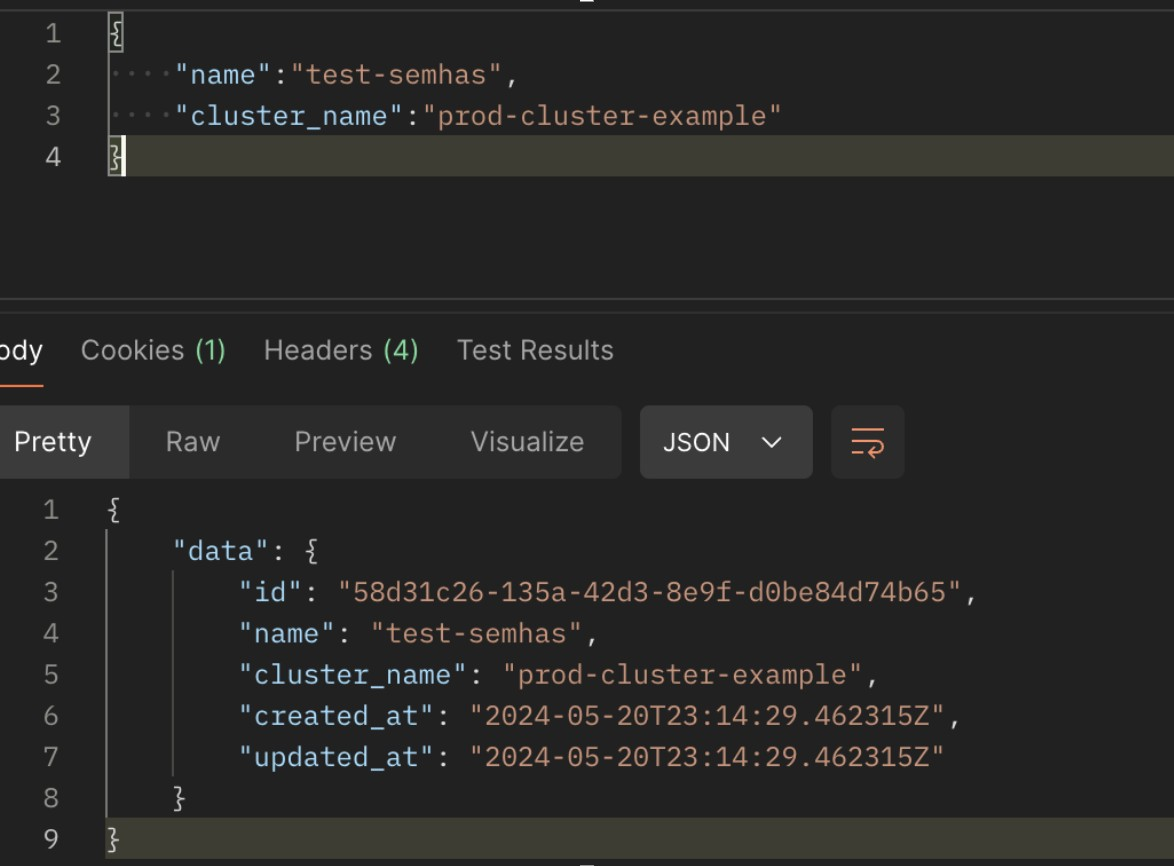
\includegraphics[width=0.8\textwidth]{resources/chapter-4/pengujian/pengujian-sistem-gcp-01.jpg}
  \caption{Pembuatan \textit{Company} pada Cluster \textit{GCP}}
  \label{fig:pengujian-sistem-gcp-01}
\end{figure}

\begin{figure}[ht]
  \centering
  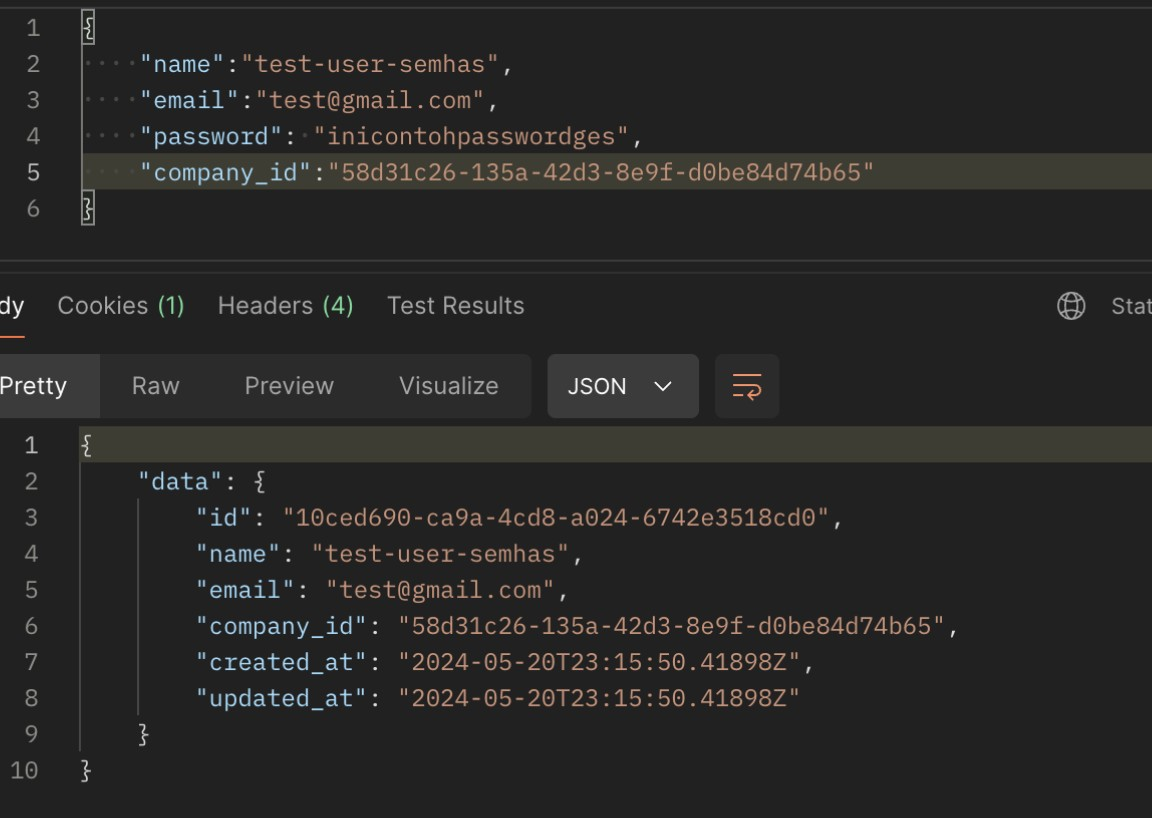
\includegraphics[width=0.8\textwidth]{resources/chapter-4/pengujian/pengujian-sistem-gcp-02.jpg}
  \caption{Pembuatan \textit{User} pada Cluster \textit{GCP}}
  \label{fig:pengujian-sistem-gcp-02}
\end{figure}

\begin{figure}[ht]
  \centering
  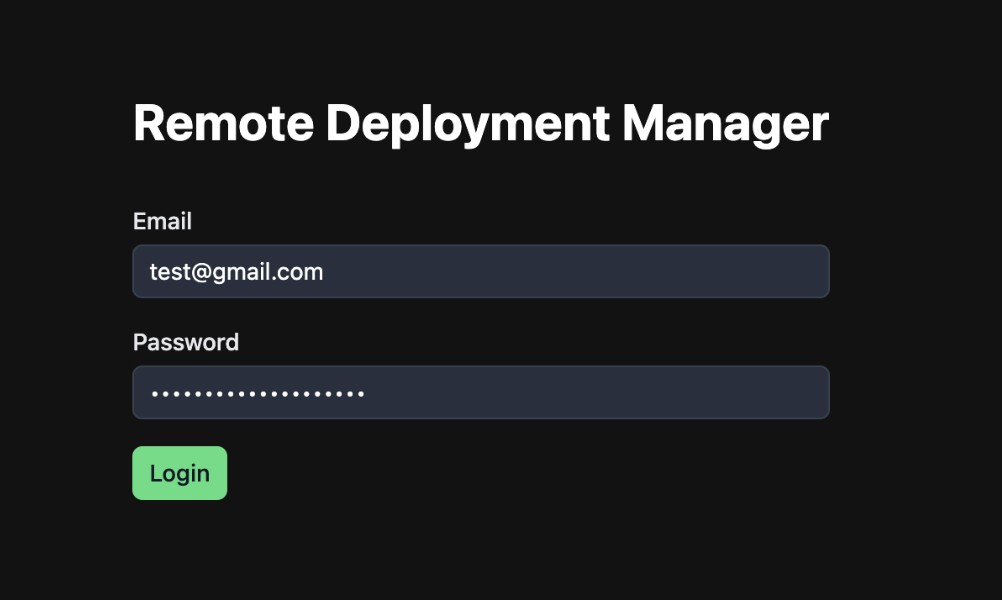
\includegraphics[width=0.8\textwidth]{resources/chapter-4/pengujian/pengujian-sistem-gcp-03.jpg}
  \caption{\textit{User} Sukses Melakukan Login}
  \label{fig:pengujian-sistem-gcp-03}
\end{figure}

\begin{figure}[ht]
  \centering
  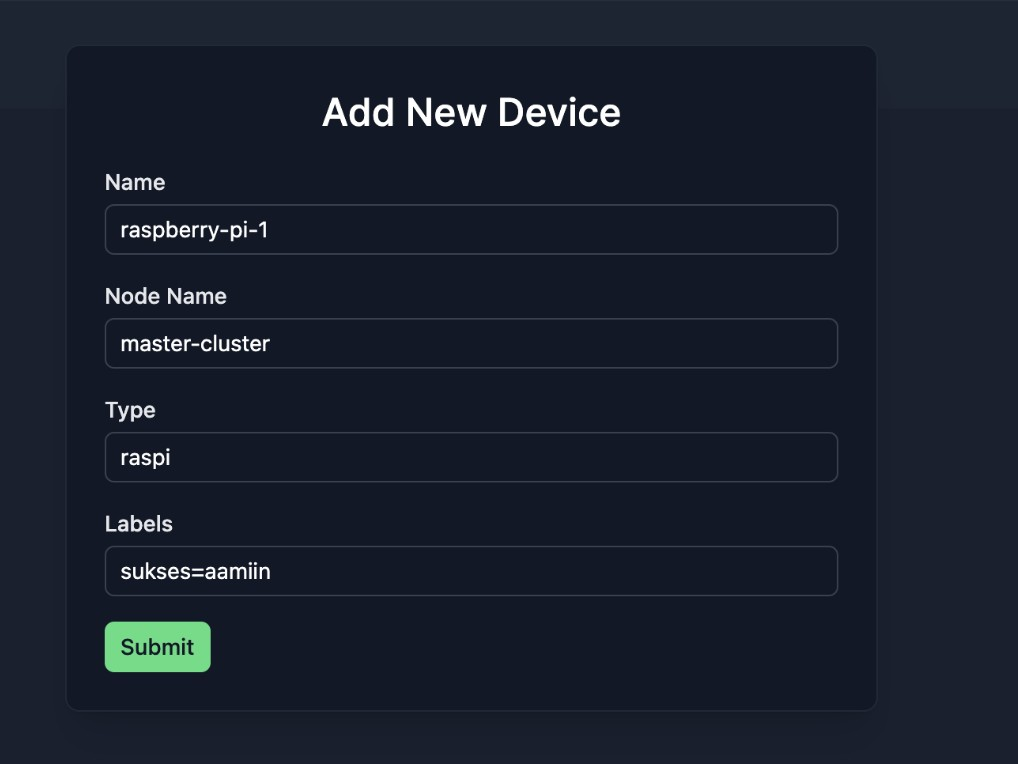
\includegraphics[width=0.8\textwidth]{resources/chapter-4/pengujian/pengujian-sistem-gcp-04.jpg}
  \caption{Pembuatan \textit{Device} pada \textit{Cluster GCP}}
  \label{fig:pengujian-sistem-gcp-04}
\end{figure}

\begin{figure}[ht]
  \centering
  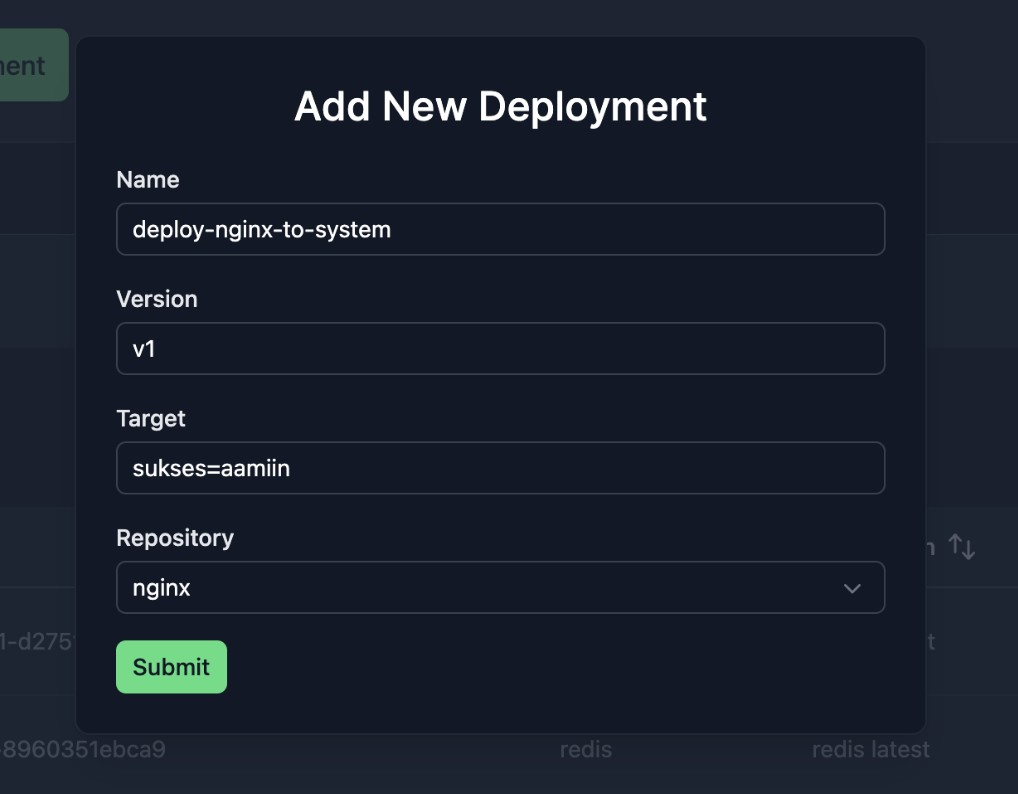
\includegraphics[width=0.8\textwidth]{resources/chapter-4/pengujian/pengujian-sistem-gcp-05.jpg}
  \caption{Pembuatan \textit{Deployment Plan} pada \textit{Cluster GCP}}
  \label{fig:pengujian-sistem-gcp-05}
\end{figure}

\begin{figure}[ht]
  \centering
  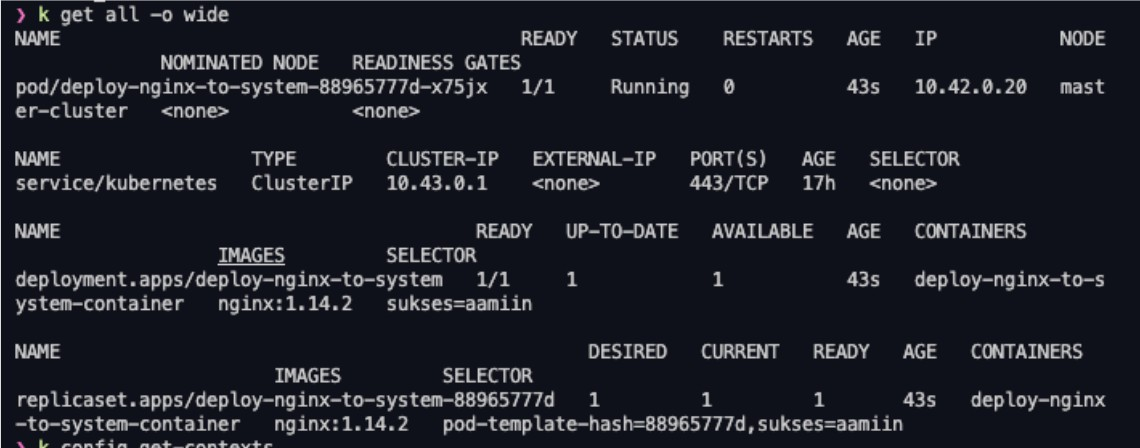
\includegraphics[width=0.8\textwidth]{resources/chapter-4/pengujian/pengujian-sistem-gcp-06.jpg}
  \caption{Hasil \textit{Remote Deployment} pada \textit{Cluster GCP}}
  \label{fig:pengujian-sistem-gcp-06}
\end{figure}

\begin{figure}[ht]
  \centering
  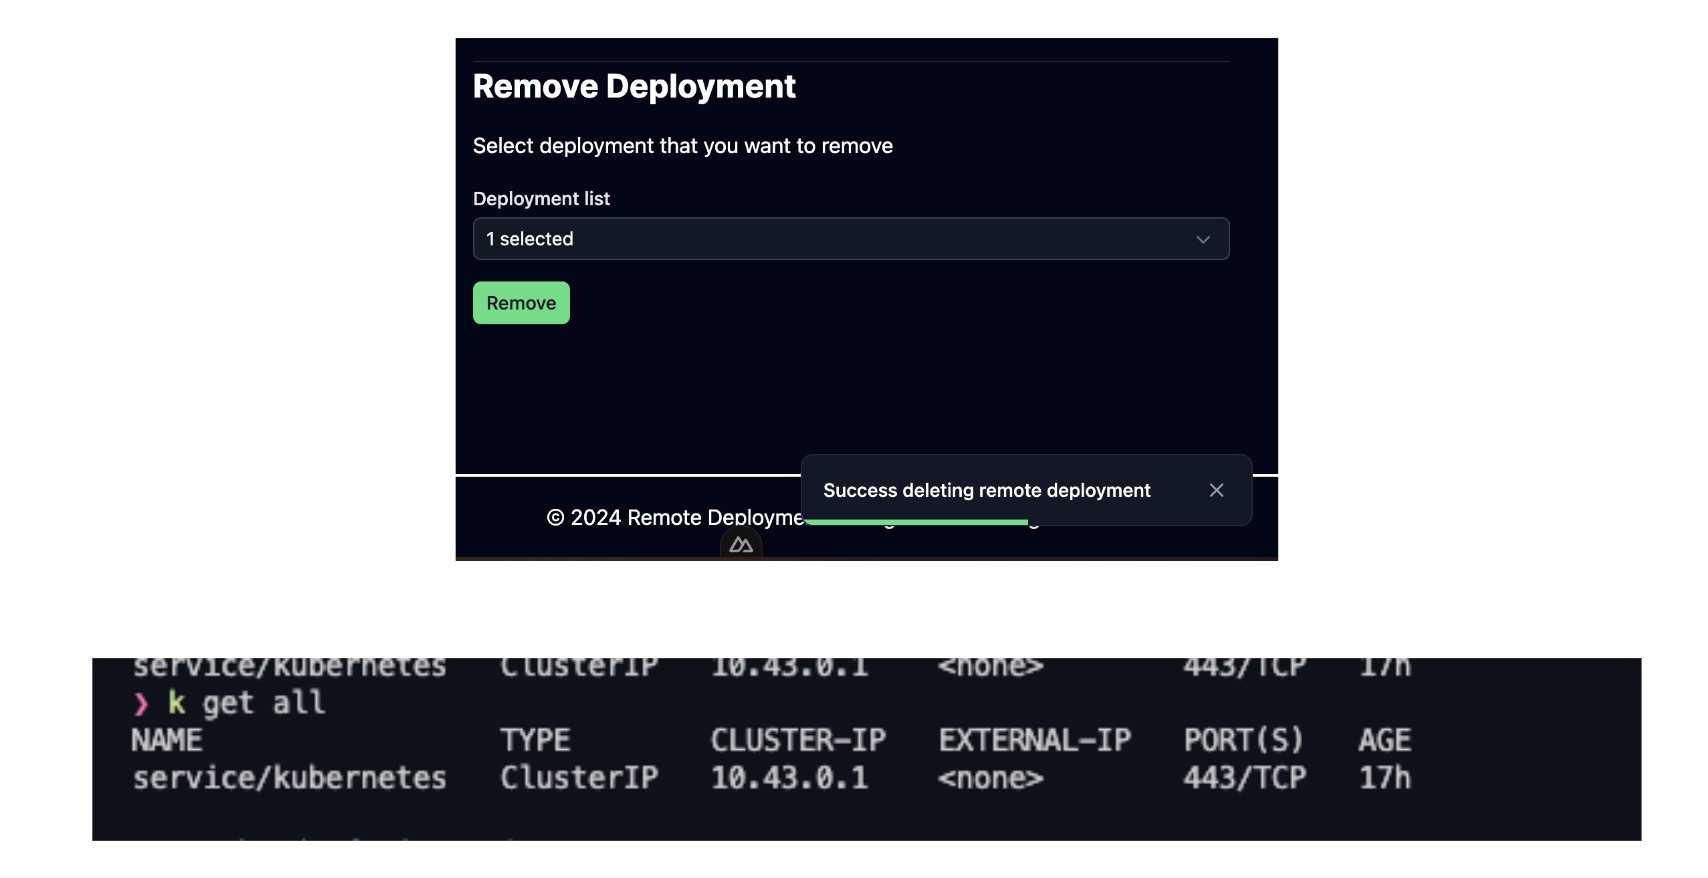
\includegraphics[width=0.8\textwidth]{resources/chapter-4/pengujian/pengujian-sistem-gcp-07.jpg}
  \caption{Hasil Penghapusan \textit{Remote Deployment} pada \textit{Cluster GCP}}
  \label{fig:pengujian-sistem-gcp-07}
\end{figure}

\begin{figure}[ht]
  \centering
  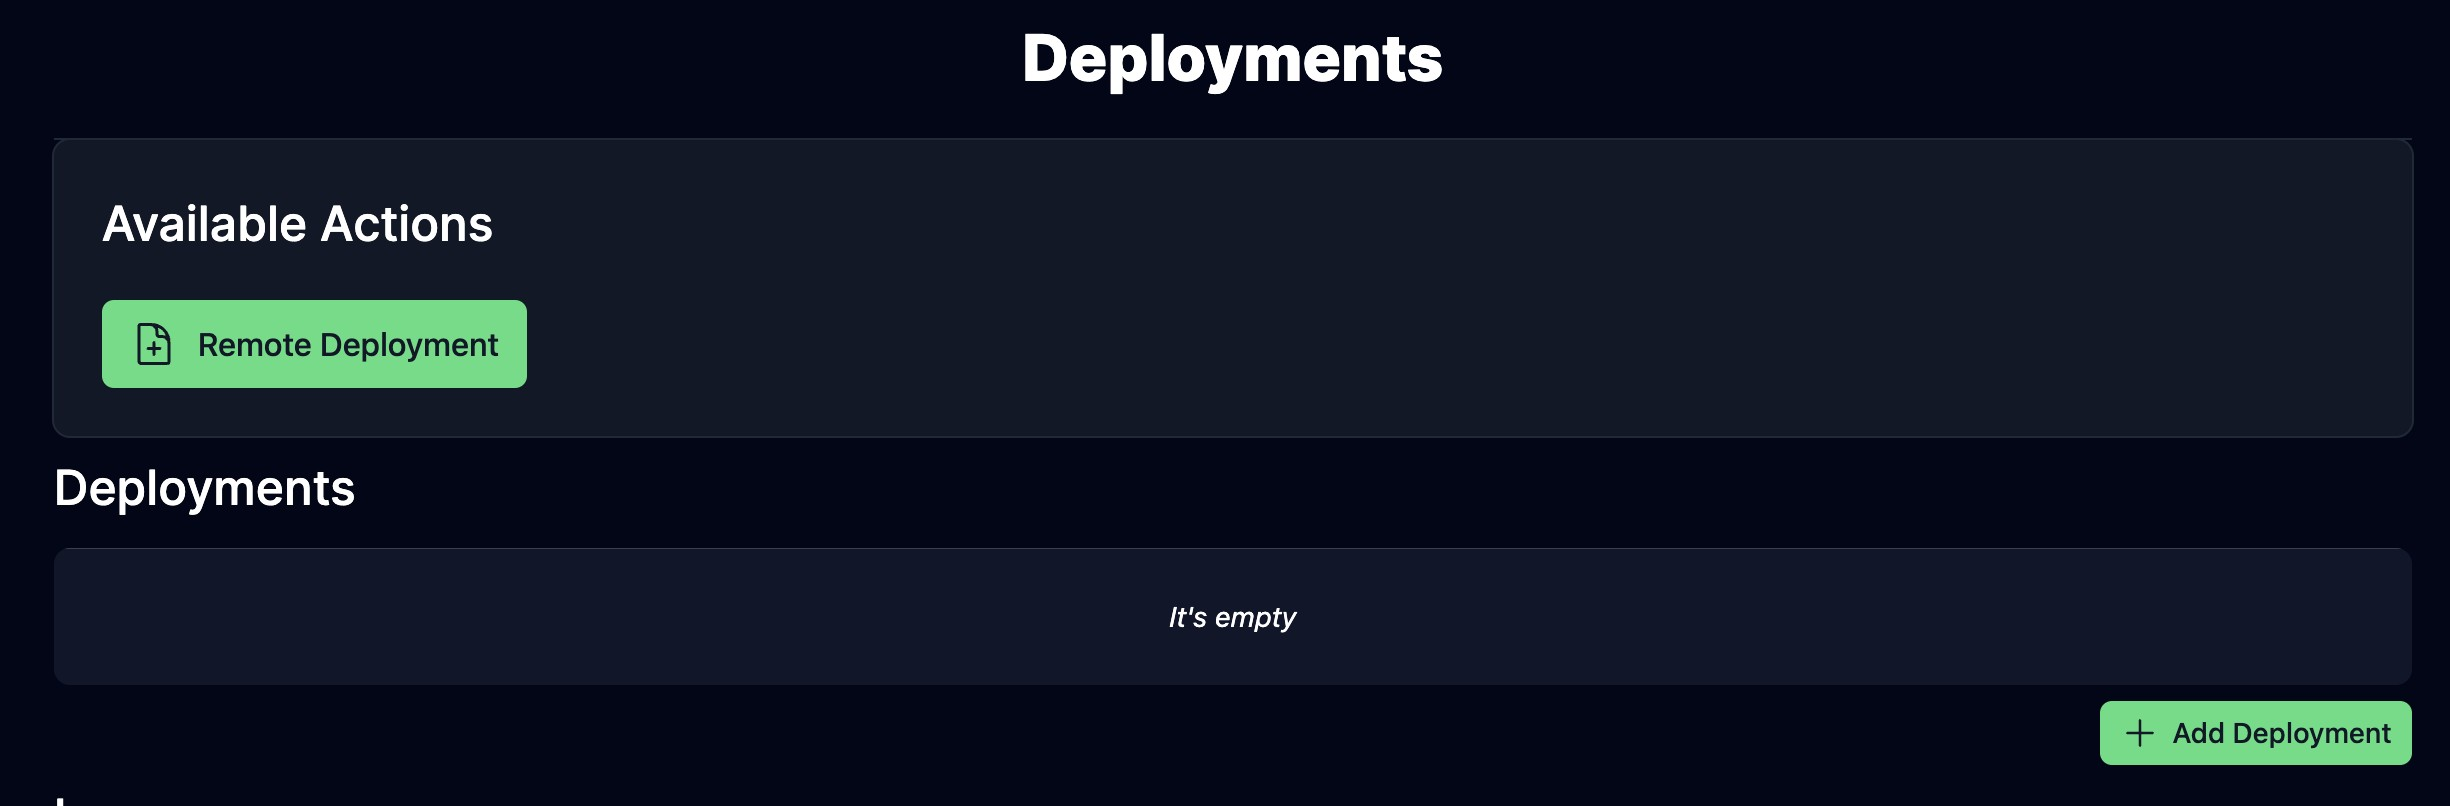
\includegraphics[width=0.8\textwidth]{resources/chapter-4/pengujian/pengujian-sistem-gcp-08.jpg}
  \caption{Hasil Penghapusan \textit{Deployment Plan} pada \textit{Cluster GCP}}
  \label{fig:pengujian-sistem-gcp-08}
\end{figure}

\begin{figure}[ht]
  \centering
  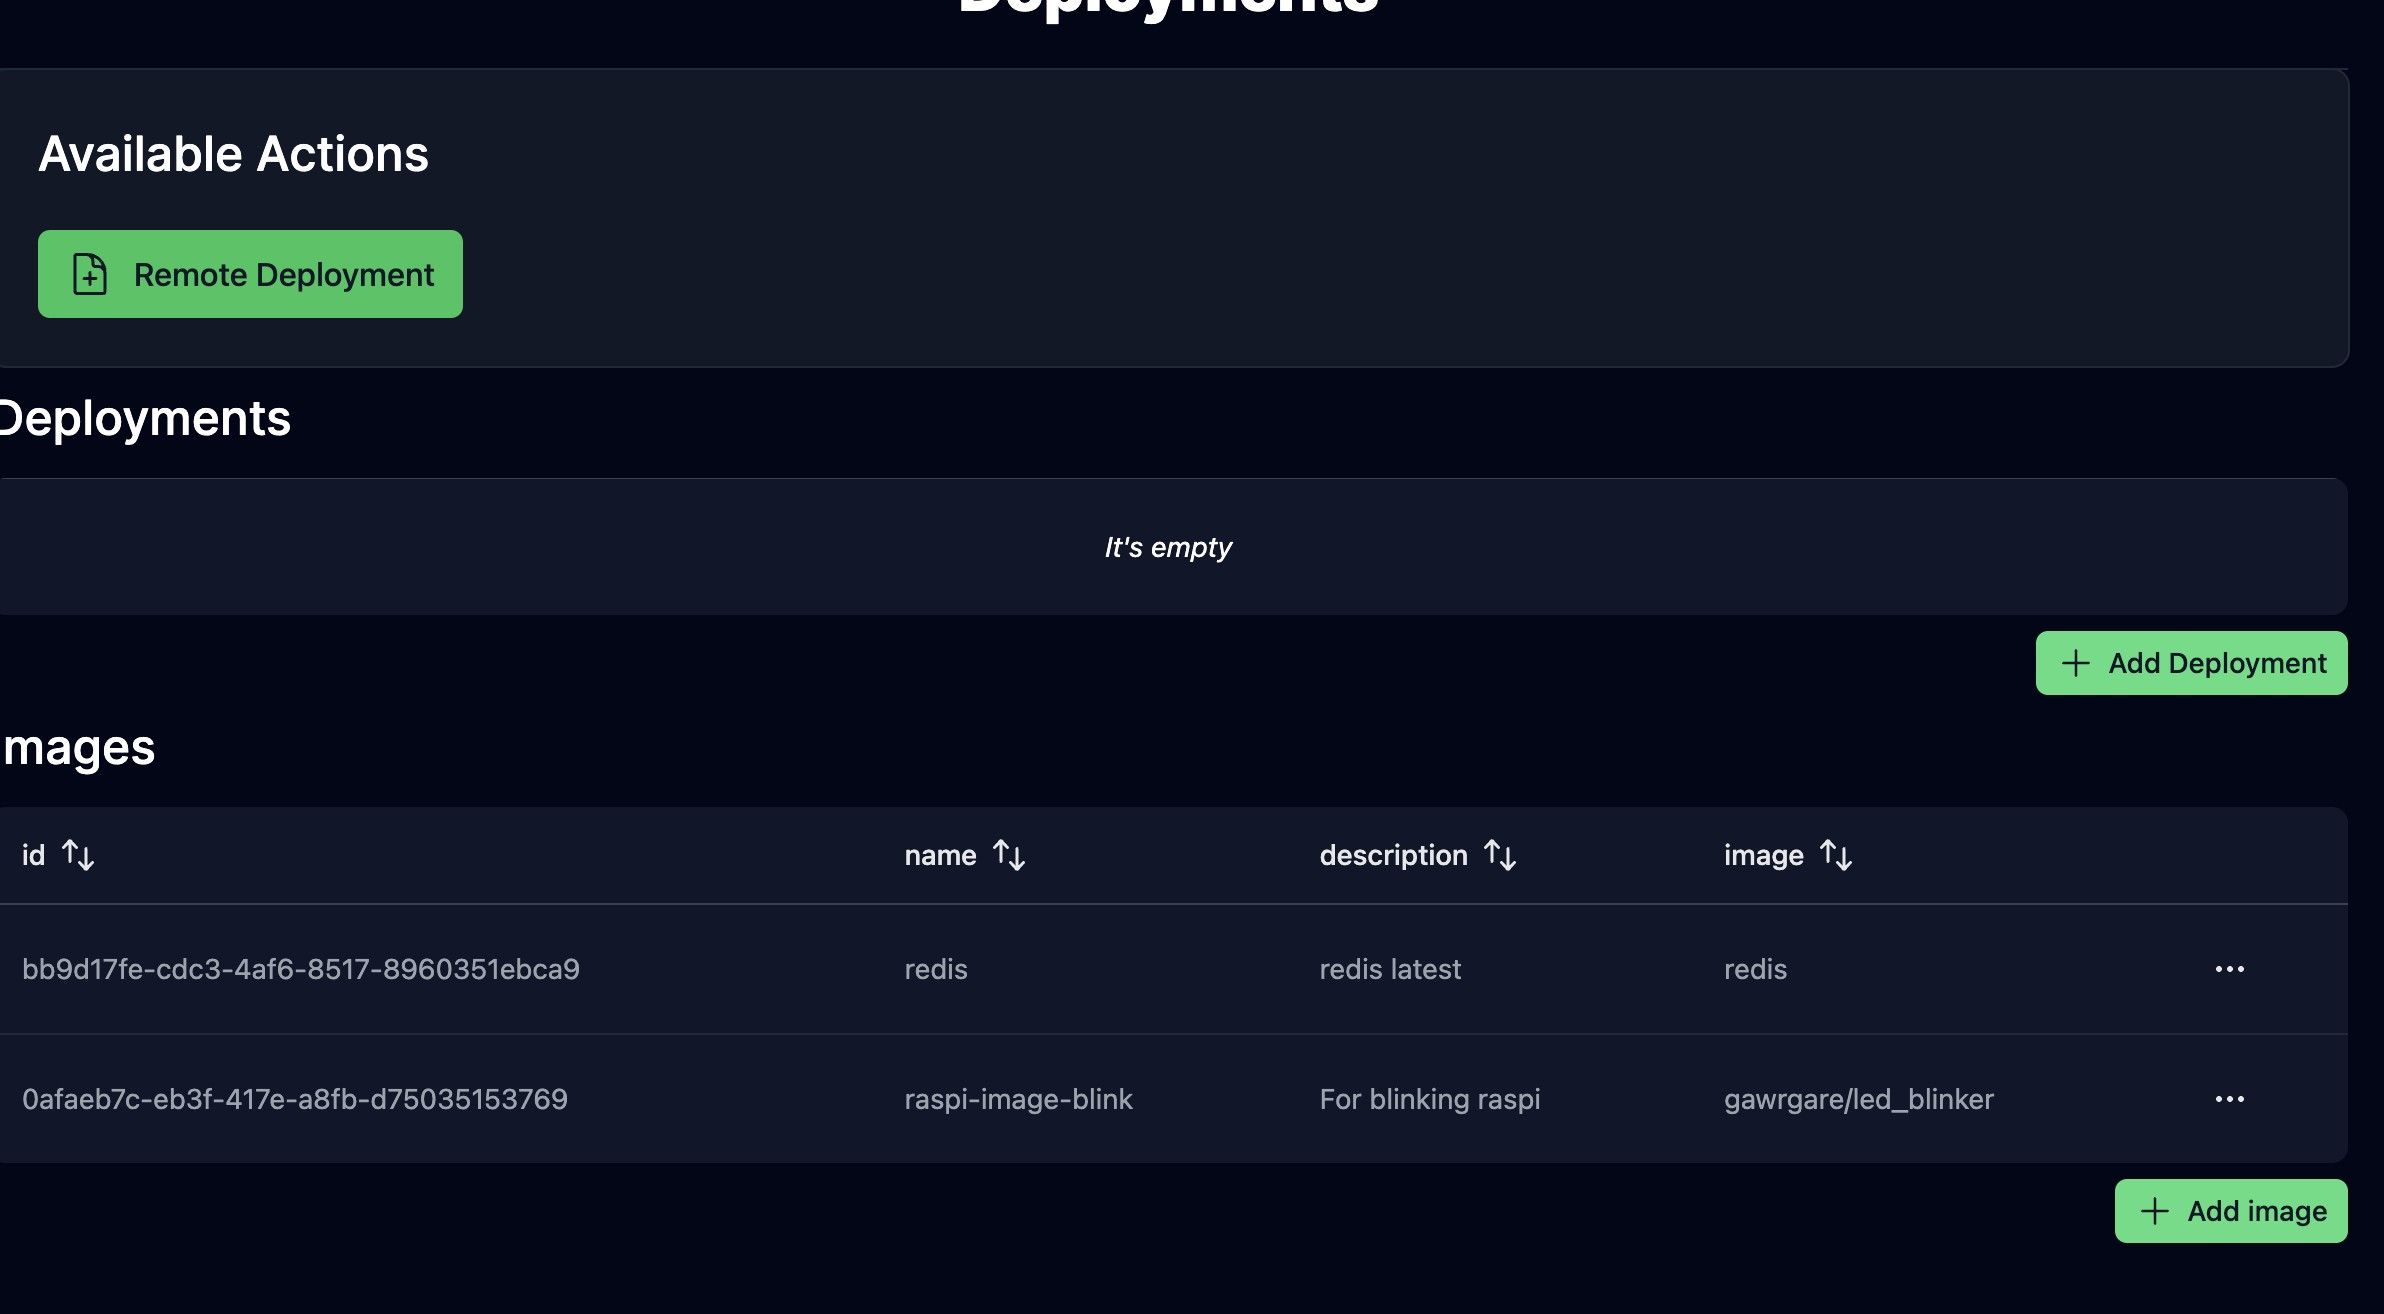
\includegraphics[width=0.8\textwidth]{resources/chapter-4/pengujian/pengujian-sistem-gcp-09.jpg}
  \caption{Hasil Penghapusan \textit{Deployment Images} pada \textit{Cluster GCP}}
  \label{fig:pengujian-sistem-gcp-09}
\end{figure}

\bgroup
\begin{table}[ht]
  \def\arraystretch{1.3}
  \caption{Skenario dan Hasil Pengujian Sistem pada \textit{Cluster GCP}}
  \label{tab:pengujian-sistem-gcp}
  \centering
  \begin{tabular}{|p{2cm}|p{2cm}|p{4cm}|p{3cm}|p{2cm}|}
    \hline
    \centering{ID Fungsional} & \centering{ID Pengujian} & \centering{Skenario}                                                                                        & \centering{Ekspektasi}                                & Realita \\
    \hline
    F01                       & P32                      & \textit{Admin} membuat \textit{company} yang dengan nama "test-semhas"                                      & \textit{Admin} berhasil mendaftarkan \textit{company} & Sesuai  \\
    \hline
    F04                       & P33                      & \textit{Admin} membuat \textit{user} yang dengan email "test@gmail.com"                                     & \textit{Admin} berhasil mendaftarkan \textit{user}    & Sesuai  \\
    \hline
    F06                       & P34                      & \textit{User} ingin login dengan kredensial "test@gmail.com"                                                & \textit{User} berhasil login ke dalam sistem          & Sesuai  \\
    \hline
    F10                       & P35                      & \textit{User} mendaftarkan \textit{device} dengan nama "raspberrypi-pi-1" dengan nama node "master-cluster" & \textit{User} berhasil mendaftarkan \textit{device}   & Sesuai  \\
    \hline
  \end{tabular}
\end{table}
\egroup

\bgroup
\begin{table}[ht]
  \def\arraystretch{1.3}
  \centering
  \begin{tabular}{|p{2cm}|p{2cm}|p{4cm}|p{3cm}|p{2cm}|}
    \hline
    \centering{ID Fungsional} & \centering{ID Pengujian} & \centering{Skenario}                                                                                          & \centering{Ekspektasi}                                            & Realita \\
    \hline

    F18                       & P36                      & \textit{User} melihat daftar \textit{deployment images} yang tersedia dengan mengunjungi halaman /deployments & \textit{User} berhasil melihat daftar \textit{deployment images}  & Sesuai  \\
    \hline
    F20                       & P37                      & \textit{User} membuat \textit{deployment plan} dengan nama "deploy-nginx-to-system"                           & \textit{User} berhasil membuat \textit{deployment plan}           & Sesuai  \\
    \hline
    F22                       & P38                      & \textit{User} menghapus \textit{deployment plan} dengan nama "deploy-nginx-to-system"                         & \textit{User} berhasil melihat menghapus \textit{deployment plan} & Sesuai  \\
    \hline
    F19                       & P39                      & \textit{User} menghapus \textit{deployment images} dengan nama NGINX                                          & \textit{User} berhasil menghapus \textit{deployment images}       & Sesuai  \\
    \hline
  \end{tabular}
\end{table}
\egroup